\documentclass[@BEAMER_OPTIONS@]{beamer}
    @USE_PGFPAGES@

    \usetheme[alternativetitlepage=true,titleline=true]{Torino}
    \setbeamertemplate{navigation symbols}{}
    \setbeamertemplate{note page}[plain]

    \usepackage[utf8]{inputenc}
    \usepackage{graphicx}
    \usepackage{subfigure}
    \usepackage{xspace}
    \usepackage{adjustbox}
    \usepackage{tikz}
    \usepgflibrary{arrows}
    \usetikzlibrary{shadows,decorations.pathreplacing,patterns,shapes}
    \tikzstyle{every picture}=[semithick,>=stealth,remember picture]
    \usepackage{listings}
    \lstset{
        language=C++,
        basicstyle=\footnotesize\rmfamily,
        stringstyle=\color{chameleon4},
        numbers=left,
        numberstyle=\tiny,
        aboveskip=-0.02\baselineskip,
        belowskip=-0.02\baselineskip,
        columns=flexible,
        extendedchars=false,
        showstringspaces=false,
        morekeywords={global,kernel,ulong,size_t,get_global_id,get_global_size}
        }
    \newcommand{\code}[1]{\lstinline|#1|}
    \newcommand{\additive}{\hspace{1cm}\footnotesize(\emph{Additive expressions only})}
    \newcommand{\plusplus}{{\nolinebreak[4]\hspace{-.05em}\raisebox{.4ex}{\tiny\bf ++}}\xspace}
    \newcommand{\Cpp}{C\plusplus}
    \newcommand{\ghribbon}{
        \begin{tikzpicture}[remember picture,overlay]
            \node[anchor=north east,yshift=4pt,xshift=4pt] at (current page.north east) {
                \href{https://github.com/ddemidov/vexcl}{\includegraphics[width=2cm]{forkme}}
            };
        \end{tikzpicture}
    }

    \title{VexCL -- Automatic OpenCL Code Generation}

    \author{Denis Demidov}
    \institute{
        Supercomputer Center of Russian Academy of Sciences \\
        Kazan Federal University
    }
    \date{October 2013, Austin, Texas}

\begin{document}

%----------------------------------------------------------------------------
\begin{frame}{}
    \titlepage
\end{frame}

\note{ }

%----------------------------------------------------------------------------
\begin{frame}{}
    \tableofcontents
\end{frame}

\note{ }

\section{Expression templates}

%----------------------------------------------------------------------------
\begin{frame}{Expression templates}
    \begin{itemize}
        \item How to implement a DSL in \Cpp \emph{effectively}?
            \vspace{\baselineskip}
        \item The idea is quite old:
            \begin{itemize}
                \item \emph{Todd Veldhuizen}, Expression templates, \Cpp Report,
                    \alert{1995}
            \end{itemize}
        \item First (?) implementation:
            \begin{itemize}
                \item Blitz\plusplus \emph{is a \Cpp class library for scientific
                computing which provides performance\\
                on par with Fortran 77/90}.
            \end{itemize}
        \item Today:
            \begin{itemize}
                \item std::valarray, Boost.uBLAS, MTL, Eigen, Armadillo, etc.
            \end{itemize}
            \vspace{\baselineskip}
        \item \emph{How does it work?}
    \end{itemize}
\end{frame}

\note{ }

%----------------------------------------------------------------------------
\begin{frame}[fragile]{Simple example: Vector addition}
    \begin{exampleblock}{We want to be able to write:}
        \begin{lstlisting}
x = y + z;
        \end{lstlisting}
    \end{exampleblock}

    \begin{exampleblock}{And it has to be as effective as:}
        \begin{lstlisting}
for(size_t i = 0; i < n; ++i)
    x[i] = y[i] + z[i];
        \end{lstlisting}
    \end{exampleblock}
\end{frame}

\note{ }

%----------------------------------------------------------------------------
\begin{frame}[fragile]{\Cpp allows us to overload operators!}
    \begin{exampleblock}{}
        \begin{lstlisting}
const vector operator+(const vector &a, const vector &b) {
    assert(a.size() == b.size());
    vector c( a.size() );
    for(size_t i = 0; i < a.size(); ++i)
        c[i] = a[i] + b[i];
    return c;
}
        \end{lstlisting}
    \end{exampleblock}
    \begin{itemize}
        \item<2-> Any problems?
            \begin{itemize}
                \item<3-> Extra memory allocation
                \item<4-> Extra memory I/O
            \end{itemize}
    \end{itemize}
\end{frame}

\note{ }

%----------------------------------------------------------------------------
\begin{frame}[fragile]{Lazy evaluation v0.1}
    \begin{exampleblock}{}
        \begin{lstlisting}
struct vsum {
    const vector &a;
    const vector &b;
    vsum(const vector &a, const vector &b) : a(a), b(b) {}
};
        \end{lstlisting}
        \pause
        \begin{lstlisting}[firstnumber=last]

const vsum operator+(const vector &a, const vector &b) {
    return vsum(a, b);
}
        \end{lstlisting}
        \pause
        \begin{lstlisting}[firstnumber=last]

const vector& vector::operator=(const vsum &s) {
    for(size_t i = 0; i < data.size(); ++i)
        data[i] = s.a[i] + s.b[i];
    return *this;
}
        \end{lstlisting}
    \end{exampleblock}
\end{frame}

\note{ }

%----------------------------------------------------------------------------
\begin{frame}[fragile]{Not general enough}
    \begin{exampleblock}{What happens if we write this?}
        \begin{lstlisting}
a = x + y + z;
        \end{lstlisting}
    \end{exampleblock}

    \begin{exampleblock}<2>{}
        \begin{verbatim}
lazy_v1.cpp:38:15: error: invalid operands to binary expression
      ('const vsum' and 'vector')
    a = x + y + z;
        ~~~~~ ^ ~
lazy_v1.cpp:12:12: note: candidate function not viable:
      no known conversion from 'const vsum'
      to 'const vector' for 1st argument
const vsum operator+(const vector &a, const vector &b) {
           ^
1 error generated.
        \end{verbatim}
    \end{exampleblock}
    \begin{description}
        \item<2>[Sidenote:] Clang error messages are awesome!
    \end{description}
\end{frame}

\note{ }

%----------------------------------------------------------------------------
\begin{frame}[fragile,shrink=2]{Lazy evaluation v0.2}
    \begin{exampleblock}{}
        \begin{lstlisting}
template <class LHS, class RHS>
struct vsum {
    const LHS &lhs;
    const RHS &rhs;
    vsum(const LHS &lhs, const RHS &rhs) : lhs(lhs), rhs(rhs) {}
    double operator[](size_t i) const {
        return lhs[i] + rhs[i];
    }
};
        \end{lstlisting}
        \pause
        \begin{lstlisting}[firstnumber=last]

template <class LHS, class RHS>
const vsum<LHS, RHS> operator+(const LHS &a, const RHS &b) {
    return vsum<LHS, RHS>(a, b);
}
        \end{lstlisting}
        \pause
        \begin{lstlisting}[firstnumber=last]

template<class Expr>
const vector& vector::operator=(const Expr &expr) {
    for(int i = 0; i < data.size(); ++i) data[i] = expr[i];
    return *this;
}
        \end{lstlisting}
    \end{exampleblock}
\end{frame}

\note{ }

%----------------------------------------------------------------------------
\begin{frame}{Still not general enough}
    \begin{itemize}
        \item There are times in life when addition alone is not enough\ldots
    \end{itemize}
\end{frame}

\note{ }

%----------------------------------------------------------------------------
\begin{frame}[fragile]{Lazy evaluation v0.3}
    \begin{exampleblock}{}
        \begin{lstlisting}
struct plus {
    static double apply(double a, double b) { return a + b; }
};
        \end{lstlisting}
        \pause
        \begin{lstlisting}[firstnumber=last]

template <class LHS, class OP, class RHS>
struct binary_op {
    const LHS &lhs;
    const RHS &rhs;
    binary_op(const LHS &lhs, const RHS &rhs) : lhs(lhs), rhs(rhs) {}
    double operator[](size_t i) const {
        return OP::apply(lhs[i], rhs[i]);
    }
};
        \end{lstlisting}
        \pause
        \begin{lstlisting}[firstnumber=last]

template <class LHS, class RHS>
const binary_op<LHS, plus, RHS> operator+(const LHS &a, const RHS &b) {
    return binary_op<LHS, plus, RHS>(a, b);
}
        \end{lstlisting}
    \end{exampleblock}
\end{frame}

\note{ }

%----------------------------------------------------------------------------
\begin{frame}[fragile]{Expression templates are trees}
    \begin{columns}
        \begin{column}{0.45\textwidth}
            \begin{exampleblock}{The expression in the RHS of:}
                \begin{onlyenv}<1>
                    \begin{lstlisting}
a = x + y;
                    \end{lstlisting}
                \end{onlyenv}
                \begin{onlyenv}<2->
                    \begin{lstlisting}
a = x + y - z;
                    \end{lstlisting}
                \end{onlyenv}
            \end{exampleblock}
            \begin{exampleblock}{... is of type:}
                \begin{uncoverenv}<2->
                    \begin{lstlisting}[numbers=none]
binary_op<
                    \end{lstlisting}
                \end{uncoverenv}
                \begin{lstlisting}[numbers=none]
    binary_op<
        vector,
        plus,
        vector
    >
                \end{lstlisting}
                \begin{uncoverenv}<2->
                    \begin{lstlisting}[numbers=none]
    , minus
    , vector
>
                    \end{lstlisting}
                \end{uncoverenv}
            \end{exampleblock}
        \end{column}
        \begin{column}{0.45\textwidth}
            \begin{figure}
                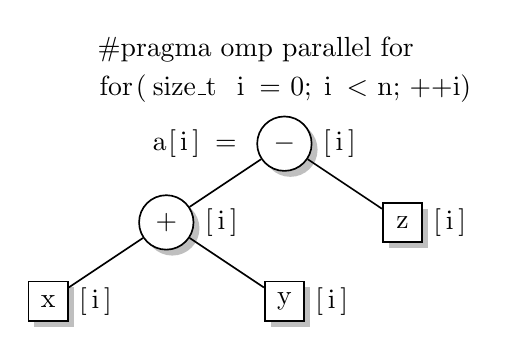
\begin{tikzpicture}
                    \uncover<2->{
                    \draw (0,0) node(sub)            [draw,fill=white,circle,drop shadow]{$-$};
                    \draw (sub) +( 1.50,-1) node(z)  [draw,fill=white,drop shadow,minimum size=0.5cm]{z};
                    }
                    \draw (sub) +(-1.50,-1) node(add)[draw,fill=white,circle,drop shadow]{$+$};
                    \draw (add) +(-1.50,-1) node(x)  [draw,fill=white,drop shadow,minimum size=0.5cm]{x};
                    \draw (add) +( 1.50,-1) node(y)  [draw,fill=white,drop shadow,minimum size=0.5cm]{y};

                    \uncover<2->{
                    \draw (sub) -- (add);
                    \draw (sub) -- (z);
                    }
                    \draw (add) -- (x);
                    \draw (add) -- (y);

                    \uncover<6>{
                        \draw (sub) +(-2.5, 1.2) node[anchor=west]{\code{#pragma omp parallel for}};
                    }
                    \uncover<3->{
                        \draw (sub) +(-2.5, 0.7) node[anchor=west]{\code{for(size_t i = 0; i < n; ++i)}};
                        \draw (sub) +(-1.8, 0.0) node[anchor=west]{\code{a[i] =}};
                    }
                    \uncover<3> {\draw (sub) +(0.7, 0) node{\code{[i]}};}
                    \uncover<4> {\draw (add) +(0.7, 0) node{\code{[i]}};}
                    \uncover<4->{\draw (z)   +(0.6, 0) node{\code{[i]}};}
                    \uncover<5->{\draw (x)   +(0.6, 0) node{\code{[i]}};}
                    \uncover<5->{\draw (y)   +(0.6, 0) node{\code{[i]}};}
                \end{tikzpicture}
            \end{figure}
        \end{column}
    \end{columns}
\end{frame}

\note{ }

%----------------------------------------------------------------------------
\begin{frame}[fragile]{So far, so good}
    \begin{exampleblock}{It is now possible to:}
        \begin{lstlisting}
v = a * x + b * y;

double c = (x + y)[42];
        \end{lstlisting}
    \end{exampleblock}

    \begin{exampleblock}{... and its as effective as:}
        \begin{lstlisting}
for(size_t i = 0; i < n; ++i)
    v[i] = a[i] * x[i] + b[i] * y[i];

double c = x[42] + y[42];
        \end{lstlisting}
    \end{exampleblock}
    \begin{itemize}
        \item No temporaries involved.
        \item Optimizing compiler is able to inline everything.
    \end{itemize}
\end{frame}

\section{OpenCL code generation}

\begin{frame}{}
    \tableofcontents[currentsection]
\end{frame}

\note{ }

%----------------------------------------------------------------------------
\begin{frame}{How does OpenCL work?}
    \begin{enumerate}
        \item A compute kernel is compiled at runtime from C99 source.
        \item Kernel parameters are set through API calls.
        \item Kernel is launched on a compute device.
    \end{enumerate}
    \vspace{\baselineskip}
    \pause
    \begin{itemize}
        \item Source may be read from a file, or stored in a static
            string, or \alert{\emph{generated}}.
    \end{itemize}
\end{frame}

\note{ }

%----------------------------------------------------------------------------
\begin{frame}[fragile]{Generating kernel source from an expression}
    \begin{exampleblock}{We want this expression:}
        \begin{lstlisting}
a = x + y - z;
        \end{lstlisting}
    \end{exampleblock}
    \begin{exampleblock}{\ldots to result in this kernel:}
        \begin{lstlisting}
kernel void vexcl_vector_kernel(
    ulong n,
    global double * res,
    global double * prm1,
    global double * prm2,
    global double * prm3
)
{
    for(size_t idx = get_global_id(0); idx < n; idx += get_global_size(0)) {
        res[idx] = ( ( prm1[idx] + prm2[idx] ) - prm3[idx] );
    }
}
        \end{lstlisting}
    \end{exampleblock}
    \begin{tikzpicture}[overlay,scale=0.8]
        \draw (11,6) node(sub)[draw,fill=white,ellipse,drop shadow]{$-$};
        \draw (sub) +( 1.50,-1) node(z)  [draw,fill=white,drop shadow,minimum size=0.5cm]{z};
        \draw (sub) +(-1.50,-1) node(add)[draw,fill=white,circle,drop shadow]{$+$};
        \draw (add) +(-1.50,-1) node(x)  [draw,fill=white,drop shadow,minimum size=0.5cm]{x};
        \draw (add) +( 1.50,-1) node(y)  [draw,fill=white,drop shadow,minimum size=0.5cm]{y};
        \draw (sub) -- (add);
        \draw (sub) -- (z);
        \draw (add) -- (x);
        \draw (add) -- (y);
    \end{tikzpicture}
\end{frame}

\note{ }

%----------------------------------------------------------------------------
\begin{frame}[fragile]{Declaring parameters}
    \begin{exampleblock}{Each terminal knows what parameters it needs:}
        \begin{lstlisting}
/*static*/ void vector::prm_decl(std::ostream &src, unsigned &pos) {
    src << ",\n    global double * prm" << ++pos;
}
        \end{lstlisting}
    \end{exampleblock}
    \begin{exampleblock}{An expression just asks its terminals to do the work:}
        \begin{lstlisting}[firstnumber=last]
template <class LHS, class OP, class RHS>
/*static*/ void binary_op<LHS, OP, RHS>::prm_decl(
                            std::ostream &src, unsigned &pos)
{
    LHS::prm_decl(src, pos);
    RHS::prm_decl(src, pos);
}
        \end{lstlisting}
    \end{exampleblock}
\end{frame}

\note{ }

%----------------------------------------------------------------------------
\begin{frame}[fragile]{Building expression string}
    \begin{exampleblock}{}
        \begin{lstlisting}
struct plus {
    static std::string string() { return "+"; }
};
        \end{lstlisting}
        \pause
        \begin{lstlisting}[firstnumber=last]

/*static*/ void vector::make_expr(std::ostream &src, unsigned &pos) {
    src << "prm" << ++pos << "[idx]";
}
        \end{lstlisting}
        \pause
        \begin{lstlisting}[firstnumber=last]

template <class LHS, class OP, class RHS>
/*static*/ void binary_op<LHS, OP, RHS>::make_expr(
                            std::ostream &src, unsigned &pos) const
{
    src << "( ";
    LHS::make_expr(src, pos);
    src << " " << OP::string() << " ";;
    RHS::make_expr(src, pos);
    src << " )";
}
        \end{lstlisting}
    \end{exampleblock}
\end{frame}

\note{ }

%----------------------------------------------------------------------------
\begin{frame}[fragile]{Source generation}
    \setbeamercovered{transparent=40}
    \begin{exampleblock}{}
        \begin{uncoverenv}<1>
            \begin{lstlisting}
template <class LHS, class RHS>
std::string kernel_source() {
    std::ostringstream src;

    src << "kernel void vexcl_vector_kernel(\n    ulong n";
            \end{lstlisting}
        \end{uncoverenv}
        \begin{uncoverenv}<1,2>
            \begin{lstlisting}[firstnumber=last]
    unsigned pos = 0;
    LHS::prm_decl(src, pos);
    RHS::prm_decl(src, pos);
            \end{lstlisting}
        \end{uncoverenv}
        \begin{uncoverenv}<1>
            \begin{lstlisting}[firstnumber=last]
    src << ")\n{\n"
            "    for(size_t idx = get_global_id(0); idx < n; idx += get_global_size(0)) {\n"
            "        ";
            \end{lstlisting}
        \end{uncoverenv}
        \begin{uncoverenv}<1,3>
            \begin{lstlisting}[firstnumber=last]
    pos = 0;
    LHS::make_expr(src, pos); src << " = ";
    RHS::make_expr(src, pos); src << ";\n";
            \end{lstlisting}
        \end{uncoverenv}
        \begin{uncoverenv}<1>
            \begin{lstlisting}[firstnumber=last]
    src << "    }\n}\n";

    return src.str();
}
            \end{lstlisting}
        \end{uncoverenv}
    \end{exampleblock}
\end{frame}

\note{ }

%----------------------------------------------------------------------------
\begin{frame}[fragile]{Setting kernel arguments}
    \begin{exampleblock}{}
        \begin{lstlisting}
void vector::set_args(cl::Kernel &krn, unsigned &pos) {
    krn.setArg(pos++, buffer);
}

template <class LHS, class OP, class RHS>
void binary_op<LHS, OP, RHS>::set_args(cl::Kernel &krn, unsigned &pos) {
    lhs.set_args(krn, pos);
    rhs.set_args(krn, pos);
}
        \end{lstlisting}
    \end{exampleblock}
\end{frame}

\note{ }

%----------------------------------------------------------------------------
\begin{frame}[fragile]{Caching compiled kernels}
    \setbeamercovered{transparent=40}
    \begin{itemize}
        \item Each kernel is uniquely identified by its expression type:
            \begin{itemize}
                \item Expression template captures terminal types and
                    operations.
            \end{itemize}
    \end{itemize}
    \begin{exampleblock}{}
        \begin{uncoverenv}<1>
            \begin{lstlisting}
template <class Expr>
const vector& vector::operator=(const Expr &expr) {
            \end{lstlisting}
        \end{uncoverenv}
        \begin{uncoverenv}<1,2>
            \begin{lstlisting}[firstnumber=last]
    static cl::Kernel kernel = build_kernel(device, kernel_source<This, Expr>());
            \end{lstlisting}
        \end{uncoverenv}
        \begin{uncoverenv}<1>
            \begin{lstlisting}[firstnumber=last]

    unsigned pos = 0;

    kernel.setArg(pos++, size);     // n
    kernel.setArg(pos++, buffer);   // res
    expr.set_args(kernel, pos);     // other parameters

    queue.enqueueNDRangeKernel(kernel, cl::NullRange, buffer.size(), cl::NullRange);

    return *this;
}
            \end{lstlisting}
        \end{uncoverenv}
    \end{exampleblock}
\end{frame}

\note{ }

%----------------------------------------------------------------------------
\begin{frame}[fragile]{What you saw is not what you get}
    \begin{itemize}
        \item The actual implementation is a bit more complicated:
            \begin{itemize}
                \item There are unary, binary, ternary expressions.
                \item There are special terminals requiring either global or
                    local preambles.
                \item There are builtin and user-defined functions.
                \item \ldots
            \end{itemize}
        \item Boost.Proto is used to keep the code mess contained.
            \vspace{\baselineskip}
        \item But you got the general idea.
    \end{itemize}
\end{frame}

\note[itemize] {
\item You are welcome to look at the actual code for more details.
}

\section{Extending VexCL}

\begin{frame}{}
    \tableofcontents[currentsection]
\end{frame}

%----------------------------------------------------------------------------
\begin{frame}[fragile,shrink=5]{General structure of OpenCL code}
    \setbeamercovered{transparent=40}
    \begin{exampleblock}{VexCL code:}
            \begin{lstlisting}
VEX_FUNCTION( sqr, double(double, double), "return prm1 * prm1 + prm2 * prm2;" );
auto tmp = vex::make_temp<1>( x );
y = sqr( sin(tmp), cos(tmp) );
            \end{lstlisting}
    \end{exampleblock}
    \begin{exampleblock}{OpenCL code:}
        \begin{uncoverenv}<1,2>
            \begin{lstlisting}
double func1(double prm1, double prm2) {
    return prm1 * prm1 + prm2 * prm2;
}
            \end{lstlisting}
        \end{uncoverenv}
        \begin{uncoverenv}<1>
            \begin{lstlisting}[firstnumber=last]
kernel void vexcl_vector_kernel(
    ulong n,
            \end{lstlisting}
        \end{uncoverenv}
        \begin{uncoverenv}<1,3>
            \begin{lstlisting}[firstnumber=last]
    global double * res,
    global double * prm1
            \end{lstlisting}
        \end{uncoverenv}
        \begin{uncoverenv}<1>
            \begin{lstlisting}[firstnumber=last]
)
{
    for(size_t idx = get_global_id(0); idx < n; idx += get_global_size(0)) {
            \end{lstlisting}
        \end{uncoverenv}
        \begin{uncoverenv}<1,4>
            \begin{lstlisting}[firstnumber=last]
        double temp1 = prm1[idx];
            \end{lstlisting}
        \end{uncoverenv}
        \begin{uncoverenv}<1,5>
            \begin{lstlisting}[firstnumber=last]
        res[idx] = func1( ( sin( temp1 ), cos( temp1 ) ) );
            \end{lstlisting}
        \end{uncoverenv}
        \begin{uncoverenv}<1>
            \begin{lstlisting}[firstnumber=last]
    }
}
            \end{lstlisting}
        \end{uncoverenv}
    \end{exampleblock}
\end{frame}

%----------------------------------------------------------------------------
\begin{frame}{Extending VexCL (adding terminal types)}
    \begin{itemize}
        \item Each terminal should tell VexCL how to use it by specializing
            several\\ struct templates:
            \begin{itemize}
                \item Does it need global preamble?
                \item What kernel parameters does it need?
                \item Does it need local preamble?
                \item What contribution does it make to expression string?
                \item How to set kernel parameters?
            \end{itemize}
    \end{itemize}
\end{frame}

%----------------------------------------------------------------------------
\begin{frame}[fragile]{Example: element index}{\code{<vexcl/element_index.hpp>}}
    \begin{exampleblock}{}
        \begin{lstlisting}
x = sin( 2 * M_PI * vex::element_index() / n );
        \end{lstlisting}
    \end{exampleblock}
    \pause
    \begin{exampleblock}{}
        \begin{lstlisting}
namespace vex {
    struct elem_index {
        size_t offset;
        elem_index(size_t offset = 0) : offset(offset) {}
    };
        \end{lstlisting}
        \pause
        \begin{lstlisting}[firstnumber=last]

    inline boost::proto::result_of::as_expr<elem_index, vector_domain>::type
    element_index(size_t offset = 0) {
        return boost::proto::as_expr<vector_domain>( elem_index(offset) );
    }
        \end{lstlisting}
        \pause
        \begin{lstlisting}[firstnumber=last]

    namespace traits {
        template <> struct is_vector_expr_terminal< elem_index > : std::true_type {};
    }
}
        \end{lstlisting}
    \end{exampleblock}
\end{frame}

%----------------------------------------------------------------------------
\begin{frame}[fragile]{Parameter declaration}
    \setbeamercovered{transparent=40}
    \begin{exampleblock}{}
        \begin{uncoverenv}<1>
            \begin{lstlisting}
namespace vex { namespace traits {
    template <class Term>
    struct kernel_param_declaration< Term,
            \end{lstlisting}
        \end{uncoverenv}
        \begin{uncoverenv}<1,2>
            \begin{lstlisting}[firstnumber=last]
            typename std::enable_if<
                boost::proto::matches< Term, boost::proto::terminal<elem_index> >::value
            >::type
            \end{lstlisting}
        \end{uncoverenv}
        \begin{uncoverenv}<1>
            \begin{lstlisting}[firstnumber=last]
        >
    {
            \end{lstlisting}
        \end{uncoverenv}
        \begin{uncoverenv}<1,3>
            \begin{lstlisting}[firstnumber=last]
        static std::string get(
            const Term&, const cl::Device&, const std::string &prm_name,
            detail::kernel_generator_state&
            )
            \end{lstlisting}
        \end{uncoverenv}
        \begin{uncoverenv}<1,4>
            \begin{lstlisting}[firstnumber=last]
        {
            std::ostringstream s;
            s << ",\n\t" << type_name<size_t>() << " " << prm_name;
            return s.str();
        }
            \end{lstlisting}
        \end{uncoverenv}
        \begin{uncoverenv}<1>
            \begin{lstlisting}[firstnumber=last]
    };
} }
            \end{lstlisting}
        \end{uncoverenv}
    \end{exampleblock}
\end{frame}

%----------------------------------------------------------------------------
\begin{frame}[fragile]{Contribution to expression string}
    \begin{exampleblock}{}
            \begin{lstlisting}
namespace vex { namespace traits {
    template <class Term>
    struct partial_vector_expr< Term,
            \end{lstlisting}
            \begin{lstlisting}[firstnumber=last]
            typename std::enable_if<
                boost::proto::matches< Term, boost::proto::terminal<elem_index> >::value
            >::type
            \end{lstlisting}
            \begin{lstlisting}[firstnumber=last]
        >
    {
            \end{lstlisting}
            \begin{lstlisting}[firstnumber=last]
        static std::string get(
            const Term&, const cl::Device&, const std::string &prm_name,
            detail::kernel_generator_state&
            )
            \end{lstlisting}
            \begin{lstlisting}[firstnumber=last]
        {
            std::ostringstream s;
            s << "(" << prm_name << " + idx)";
            return s.str();
        }
            \end{lstlisting}
            \begin{lstlisting}[firstnumber=last]
    };
} }
            \end{lstlisting}
    \end{exampleblock}
\end{frame}

%----------------------------------------------------------------------------
\begin{frame}[fragile]{Setting kernel arguments}
    \begin{exampleblock}{}
        \begin{lstlisting}
namespace vex { namespace traits {
    template <class Term>
    struct kernel_arg_setter< Term,
            typename std::enable_if<
                boost::proto::matches< Term, boost::proto::terminal<elem_index> >::value
            >::type
        >
    {
        static void set(
            const Term &term, cl::Kernel &kernel, unsigned /*device*/,
            size_t index_offset, unsigned &position,
            detail::kernel_generator_state&
            )
        {
            kernel.setArg(position++, boost::proto::value(term).offset + index_offset);
        }
    };
} }
        \end{lstlisting}
    \end{exampleblock}
\end{frame}

%----------------------------------------------------------------------------
\begin{frame}
    \begin{center}
        \begin{Huge}
            \color{chameleon1}{Questions?}
        \end{Huge}
    \end{center}
\end{frame}

\end{document}


% vim: et
